% Reference copy extracted from optimal_long_short.tex on 2026-08-16.
% This file is a LaTeX fragment and is intentionally not included in the main manuscript.
% ============================================================
\section{Numerical Implementation and Validation}\label{sec:numerical}
% ============================================================

\subsection{Validation design and empirical parameters}

We validate survival ($k=0$) and killed moments of orders $k=1,2,3,4$, examine
Talbot-order and Monte Carlo monitoring convergence, and verify the analytical no-shorting
limit as $h_0\to\infty$. The moment representation is defined for any fixed integer order
satisfying the two tail conditions in \eqref{eq:moment-admissibility}; the numerical evidence in
this section is deliberately limited to orders zero through four. We make no numerical
stability claim for all higher orders allowed by the formal moment domain.

Time-domain quantities are recovered with the Talbot deformed-contour algorithm
\citep{Talbot1979}. The resolvent is derived first to the right of its Laplace abscissa and
then continued to nonsingular contour nodes. The Monte Carlo comparison uses a finite
monitoring grid, so it is a discretization benchmark rather than a continuous-time ground
truth.

\begin{remark}[Continuation to a Talbot contour]\label{rem:talbot-continuation}
Talbot inversion evaluates \eqref{eq:Uhat-zero} at complex $q$ reached by analytic
continuation. A valid contour deformation avoids transform poles, phase poles, and root
collisions, continuing each characteristic-root branch from its right-half-plane value at
real $q$. The sign classification in Assumption~\ref{ass:six-root} is therefore an initial
labeling, not a fresh test at every complex contour node.
\end{remark}

The Kou model and contract parameters are given in Table~\ref{tab:num-params}.
Parameters are calibrated by the penalized ECF criterion described in the accompanying
empirical-calibration note
using 540 four-hour WETH (asset~1, long collateral) and
WBTC (asset~2, short debt) log-returns on AAVE v3 Ethereum after subtracting an exponentially
weighted return mean; the drifts $\mu_i$ are adjusted for AAVE supply/borrow
APRs (see caption). At the terminal sample block, the standard-mode WETH collateral
threshold $b=0.83$ and maximum origination LTV $0.805$ impose a minimum feasible
log-buffer $h_0^{\min}=\log(0.83/0.805)\approx0.031$; no eMode category applies to
the WETH-collateral/WBTC-debt pair. WETH and WBTC have distinct downward phase rates for the validated orders
$k=0,\ldots,4$, so the generic barrier system applies in the reported calculations.
Because the first moment is weakly identified in high-frequency ECF matching,
the fitted $\mu_i$ values in Table~\ref{tab:num-params} should be read as model
price-growth normalizers rather than directional forecasts; user views can replace
them in downstream moment and liquidation calculations.

\begin{table}[ht]
\centering
\renewcommand{\arraystretch}{1.3}
\begin{tabular}{llcc}
\toprule
Group & Parameter & WETH & WBTC \\
\midrule
\multirow{9}{*}{Kou}
 & ECF price-growth normalizer $\mu_i$ & $1.194$ & $0.491$ \\
 & Log-price drift $\mu_i^X$ & $0.251$ & $-0.302$ \\
 & Model log-return drift $\E[\diff X_i]/\diff t$ & $1.105$ & $0.428$ \\
 & Empirical de-meaned log drift & $0.606$ & $0.352$ \\
 & Diffusion volatility $\sigma_i$ & $0.307$ & $0.241$ \\
 & Jump intensity $\lambda_i$ & $588.95$ & $372.95$ \\
 & Upward-jump probability $p_i$ & $0.357$ & $0.508$ \\
 & Mean upward-jump size $\eta_{i,+}$ & $0.0125$ & $0.0111$ \\
 & Mean downward-jump size $\eta_{i,-}$ & $0.00469$ & $0.00743$ \\
\midrule
\multirow{4}{*}{Correlation / contract}
 & Brownian correlation $\rho$ & \multicolumn{2}{c}{$0.858$} \\
 & WETH liquidation threshold $b$ & \multicolumn{2}{c}{$0.83$} \\
 & WETH maximum origination LTV & \multicolumn{2}{c}{$0.805$} \\
 & WETH liquidation bonus & \multicolumn{2}{c}{$5\%$} \\
\midrule
\multirow{2}{*}{Portfolio}
 & Initial price $S_{i,0}$ & $2{,}060.33$ & $75{,}060.57$ \\
 & Horizon $T$ & \multicolumn{2}{c}{$1/12$ (one month)} \\
\bottomrule
\end{tabular}
\caption{Kou model and contract parameters calibrated by penalized ECF matching to four-hour
WETH/WBTC log-returns on AAVE v3 Ethereum
(2026-02-26 -- 2026-05-27), after EWM de-meaning with span 30. Drifts adjusted
for sample-average AAVE APRs: $\mu_1 {+}{=}\, 2.1901\%\,\mathrm{yr}^{-1}$ (WETH supply),
$\mu_2 {+}{=}\, 0.3479\%\,\mathrm{yr}^{-1}$ (WBTC variable borrow). Jump intensities are
estimated under the broad calibration bound $\lambda_{\max}=5000$.
The static origination terms are queried at the terminal block $25{,}189{,}091$:
WETH threshold $b=0.83$, maximum LTV $0.805$, and liquidation bonus $5\%$, giving
$h_0^{\min}\approx0.0306$. They are terminal-block inputs, not an assumption that
governance parameters remained constant over the return window. The bonus is reported as
a contract input but does not enter the paper's zero-after-liquidation payoff convention.
Derived quantities:
$\lambda_1\chi_1+\tfrac12\sigma_1^2\approx0.943$,
$\lambda_2\chi_2+\tfrac12\sigma_2^2\approx0.793$,
$\mu_1^X\approx0.251$, $\mu_2^X\approx-0.302$. The empirical de-meaned
price-growth normalizers are $0.755$ (WETH) and $0.432$ (WBTC), so the fitted
$\mu_i$ remain weakly identified ECF normalizers rather than robust return forecasts.
Initial prices are the last aligned AAVE sample at the same terminal block.}
\label{tab:num-params}
\end{table}

\subsection{Survival, killed moments, and the no-shorting limit}

For each initial health factor $H_0=e^{h_0}$, with
$h_0\in\{h_0^{\min},0.10,0.25,0.50,0.75,1.00,1.50,2.00\}$ and
$h_0^{\min}=0.030583$, we report the survival
probability $p_{\mathrm{surv}}$ and the following conditional statistics of $\Pi_T\mid\{\tau>T\}$,
where $\mu_k:=\E[\Pi_T^k\mid\tau>T]$:
\begin{equation}\label{eq:stdmom}
\begin{aligned}
&\text{mean}:=\mu_1,\qquad
\text{variance}:=\mu_2-\mu_1^2,\\
&\text{skewness}:=\frac{\mu_3-3\mu_1\mu_2+2\mu_1^3}{(\mu_2-\mu_1^2)^{3/2}},\qquad
\text{ex.\ kurt}:=\frac{\mu_4-4\mu_1\mu_3+6\mu_1^2\mu_2-3\mu_1^4}{(\mu_2-\mu_1^2)^{2}}-3.
\end{aligned}
\end{equation}

Table~\ref{tab:killed-moments} reports the objective-independent quantities that are the
paper's primary numerical output. The identity
$M_k=p_{\mathrm{surv}}\E[\Pi_T^k\mid\tau>T]$ also provides a direct implementation
check at each buffer.

\begin{table}[ht]
\centering\small
\renewcommand{\arraystretch}{1.25}
\begin{tabular}{rrrrrr}
\toprule
$h_0$ & $p_{\mathrm{surv}}$ & $M_1$ & $M_2$
& $\E[\Pi_T\mid\tau>T]$ & $\E[\Pi_T^2\mid\tau>T]$ \\
\midrule
$0.0306$ & $0.356955$ & $0.646184$ & $1.268463$ & $1.810269$ & $3.553569$ \\
$0.1000$ & $0.766735$ & $1.111927$ & $1.755024$ & $1.450210$ & $2.288957$ \\
$0.2500$ & $0.989001$ & $1.214321$ & $1.606097$ & $1.227826$ & $1.623960$ \\
$0.5000$ & $0.999995$ & $1.168318$ & $1.426096$ & $1.168324$ & $1.426104$ \\
$1.0000$ & $1.000000$ & $1.132221$ & $1.314377$ & $1.132221$ & $1.314377$ \\
$2.0000$ & $1.000000$ & $1.112544$ & $1.259450$ & $1.112544$ & $1.259450$ \\
\bottomrule
\end{tabular}
\caption{Laplace--resolvent survival probabilities, killed raw moments, and conditional
raw moments for selected feasible buffers under Table~\ref{tab:num-params}. The first row
uses the terminal-block protocol origination bound $h_0^{\min}=\log(0.83/0.805)$. Values are generated by
\texttt{h0\_liquidation\_moment\_report}, which exposes killed and conditional outputs
separately.}
\label{tab:killed-moments}
\end{table}

As $h_0\to\infty$ the short holding $n_2\to 0$ and the portfolio converges to a unit long
position in asset $1$ (Remark~\ref{rem:no-shorting}), so all conditional statistics
converge to those of $e^{X_{1,T}}$ under $\P$:
\[
\lim_{h_0\to\infty}\mu_k = \E_\P\!\left[e^{kX_{1,T}}\right]
= \exp\!\bigl(T\,\Psi(-ik,0)\bigr).
\]
Table~\ref{tab:results} reports all statistics together with these analytical limits.

\begin{table}[ht]
\centering\small
\renewcommand{\arraystretch}{1.3}
\begin{tabular}{cc cc cccc}
\toprule
& & \multicolumn{2}{c}{$p_{\mathrm{surv}}$} & & & & \\
\cmidrule(lr){3-4}
$h_0$ & $H_0$ & Lap. & MC & Mean & Variance & Skewness & Ex.\ Kurt. \\
\midrule
$0.031$ & $1.031$ & $0.3570$ & $0.3751$ & $1.8103$ & $0.2765$ & $0.8541$ & $1.0512$ \\
$0.10$ & $1.105$ & $0.7667$ & $0.7748$ & $1.4502$ & $0.1858$ & $0.7909$ & $0.8748$ \\
$0.25$ & $1.284$ & $0.9890$ & $0.9893$ & $1.2278$ & $0.1164$ & $0.5294$ & $0.4890$ \\
$0.50$ & $1.649$ & $1.0000$ & $1.0000$ & $1.1683$ & $0.0611$ & $0.4895$ & $0.5392$ \\
$0.75$ & $2.117$ & $1.0000$ & $1.0000$ & $1.1451$ & $0.0414$ & $0.5120$ & $0.5510$ \\
$1.00$ & $2.718$ & $1.0000$ & $1.0000$ & $1.1322$ & $0.0325$ & $0.5183$ & $0.5486$ \\
$1.50$ & $4.482$ & $1.0000$ & $1.0000$ & $1.1189$ & $0.0248$ & $0.5132$ & $0.5297$ \\
$2.00$ & $7.389$ & $1.0000$ & $1.0000$ & $1.1125$ & $0.0217$ & $0.5041$ & $0.5109$ \\
\midrule
$\infty$ & $\infty$ & $1.0000$ & --- & $1.1046$ & $0.0183$ & $0.4845$ & $0.4747$ \\
\bottomrule
\end{tabular}
\caption{Laplace--resolvent conditional statistics and the no-shorting analytical limit
for the long-WETH/short-WBTC calibrated parameters (Table~\ref{tab:num-params}).
Mean, variance, skewness, and excess kurtosis are conditional on survival ($\tau>T$)
and computed via the resolvent method (Laplace); MC benchmark uses $10^5$ Euler--Poisson
paths (252 monitoring intervals over the one-month horizon, seed 42). The smallest tabulated
buffer is the exact AAVE-feasible minimum
($h_0^{\min}=0.030583$, $H_0^{\min}=1.031056$); at this value
Laplace gives $p_{\mathrm{surv}}=0.3570$
versus MC $0.3751$ --- the $1.81$ percentage-point gap reflects discrete-time MC missing intra-period
liquidation events at high jump intensity
($\lambda_1\approx589$, $\lambda_2\approx373$), not path scarcity
($\approx\!37{,}500$ surviving MC paths).
The bottom row gives the analytical limits as $h_0\to\infty$; Laplace at $h_0=100$ matches
these values to relative error $<10^{-6}$, confirming internal consistency of the
resolvent construction, Talbot inversion, and the drift normalisation
$\mu_i^X=\mu_i-\tfrac{1}{2}\sigma_i^2-\lambda_i\chi_i$.}
\label{tab:results}
\end{table}

\begin{table}[ht]
\centering\small
\renewcommand{\arraystretch}{1.3}
\begin{tabular}{cc rrrrr rr}
\toprule
& & \multicolumn{5}{c}{Laplace $-$ MC} & \multicolumn{2}{c}{CPU time (s)} \\
\cmidrule(lr){3-7}\cmidrule(lr){8-9}
$h_0$ & $H_0$ & $\Delta p_{\mathrm{surv}}$ & $\Delta$Mean & $\Delta$Var.\ & $\Delta$Skew.\ & $\Delta$Kurt.\ & Lap.\ & MC \\
\midrule
$0.031$ & $1.031$ & $-0.0181$ & $\phantom{-}0.0111$ & $\phantom{-}0.0039$ & $\phantom{-}0.0188$ & $\phantom{-}0.0505$ & $0.069$ & $51.09$ \\
$0.10$ & $1.105$ & $-0.0080$ & $\phantom{-}0.0045$ & $\phantom{-}0.0011$ & $\phantom{-}0.0257$ & $\phantom{-}0.0717$ & $0.067$ & $49.51$ \\
$0.25$ & $1.284$ & $-0.0002$ & $\phantom{-}0.0005$ & $\phantom{-}0.0004$ & $\phantom{-}0.0237$ & $\phantom{-}0.0503$ & $0.067$ & $49.62$ \\
$0.50$ & $1.649$ & $\phantom{-}0.0000$ & $\phantom{-}0.0003$ & $\phantom{-}0.0002$ & $\phantom{-}0.0189$ & $\phantom{-}0.0445$ & $0.067$ & $49.42$ \\
$0.75$ & $2.117$ & $\phantom{-}0.0000$ & $\phantom{-}0.0002$ & $\phantom{-}0.0001$ & $\phantom{-}0.0168$ & $\phantom{-}0.0397$ & $0.067$ & $49.61$ \\
$1.00$ & $2.718$ & $\phantom{-}0.0000$ & $\phantom{-}0.0002$ & $\phantom{-}0.0000$ & $\phantom{-}0.0147$ & $\phantom{-}0.0343$ & $0.067$ & $49.51$ \\
$1.50$ & $4.482$ & $\phantom{-}0.0000$ & $\phantom{-}0.0002$ & $\phantom{-}0.0000$ & $\phantom{-}0.0114$ & $\phantom{-}0.0250$ & $0.068$ & $49.83$ \\
$2.00$ & $7.389$ & $\phantom{-}0.0000$ & $\phantom{-}0.0002$ & $\phantom{-}0.0000$ & $\phantom{-}0.0094$ & $\phantom{-}0.0187$ & $0.068$ & $50.41$ \\
\bottomrule
\end{tabular}
\caption{Laplace minus MC differences ($\Delta = \text{Lap.} - \text{MC}$) and wall-clock
computation time. The persistent $\Delta p_{\mathrm{surv}}<0$ reflects the discretely
monitored Euler--Poisson scheme (252 intervals over $[0,T]$) missing intra-interval
liquidation events; the
effect is strongest near $H_0^{\min}\approx1.031$ where paths frequently approach the barrier.
Higher-moment differences shrink as $H_0$ increases and more paths survive into the interior.
The Laplace timing covers five Talbot inversions ($k=0,\ldots,4$). On the reported host it
is roughly 740 times smaller than the particular $10^5$-path MC run; this ratio is
hardware-, implementation-, path-count-, and monitoring-grid-dependent, not a universal
speed-up constant.}
\label{tab:diff}
\end{table}

\subsection{Monitoring and inversion diagnostics}

Table~\ref{tab:mc-convergence} isolates monitoring error at $h_0=0.10$. Refining the
Euler--Poisson grid moves the MC survival estimate toward the Laplace value
$0.766735$: the gap falls from $1.95$ percentage points at 63 intervals to $0.64$
percentage points at 1008 intervals. The Laplace value remains just below the reported
1008-interval binomial interval, so the finite-grid bias is not yet negligible. Refinement
does not turn the simulation into exact continuous monitoring---jump ordering and Brownian
crossings within an interval remain approximated---but the convergence direction supports
the interpretation of the coarse-grid discrepancy in Table~\ref{tab:diff}.

\begin{table}[ht]
\centering\small
\renewcommand{\arraystretch}{1.25}
\begin{tabular}{rrrrr}
\toprule
Intervals over $[0,T]$ & MC $p_{\mathrm{surv}}$ & Binomial s.e. & Approx. 95\% interval & Time (s) \\
\midrule
$63$   & $0.78624$ & $0.00259$ & $[0.78116,0.79132]$ & $10.78$ \\
$252$  & $0.77416$ & $0.00264$ & $[0.76898,0.77934]$ & $13.97$ \\
$1008$ & $0.77312$ & $0.00265$ & $[0.76793,0.77831]$ & $15.24$ \\
\bottomrule
\end{tabular}
\caption{Discrete-monitoring convergence for $h_0=0.10$, $T=1/12$, 25,000 paths,
and seed 42. The interval is the normal binomial interval for survival incidence and does
not include time-discretization uncertainty.}
\label{tab:mc-convergence}
\end{table}

For the feasible lower buffer $h_0=0.030583$, changing the Talbot order from 12 to 40
changes $p_{\mathrm{surv}}$ and $M_1,M_2$ only beyond the eighth reported decimal; the
largest relative change between $M=32$ and $M=40$ among $k=0,\ldots,4$ is
$9.4\times10^{-9}$ (for $M_4$). Over the $M=32$ contour nodes and the same orders, the
maximum relative characteristic-root residual is $1.1\times10^{-13}$, the minimum
root-to-pole distance is $3.51$, and the largest barrier-matrix condition number is $25.13$.
The maximum linear-system residual is $4.3\times10^{-18}$.

These quantities are reported by \texttt{jobs/numerical\_diagnostics.py}. The current
implementation selects the three root branches by real-part rank at each contour node rather
than by a global nearest-branch continuation algorithm. The residual, separation, pole, and
conditioning checks support that selection for this calibration and $k=0,\ldots,4$; they do
not justify extrapolation to every formally admissible higher order.

\subsection{Parameter sensitivity}\label{sec:sensitivity}

Figure~\ref{fig:sensitivity} shows how $p_{\mathrm{surv}}$ (left column) and the conditional
mean $\E[\Pi_T\mid\tau>T]$ (right column) vary with $H_0$ as each parameter is swept in turn.
For the liquidation threshold $b$ (row~e--f), survival probability is independent of $b$ at fixed
$H_0$ — only the payoff kernel changes — so the left panel shows the initial leverage
$L_0 = H_0/(H_0-b)$ instead.

Three patterns dominate. (i)~Sensitivity is concentrated near the origination boundary:
jump-intensity, volatility, correlation, and horizon variants visibly separate at low $H_0$
but their survival curves approach one as the buffer grows. At $H_0\approx1.35$, even the
$2\times$ jump-intensity, $2\times$ volatility, and three-month variants have survival above
$96\%$. (ii)~Higher jump intensity, volatility, or horizon lowers survival near the barrier
and raises the conditional mean there through selective survival; the longer horizon also
accumulates the benchmark's positive WETH-minus-WBTC drift. Correlation acts through the
effective variance of $Z=X_1-X_2$: increasing $\rho$ raises survival, while its effect on
the plotted conditional mean remains modest for this calibration. (iii)~For $b$, survival
is unchanged at fixed $H_0$, but holdings and payoff moments are not. Initial leverage
$L_0=H_0/(H_0-b)$ reaches ${\approx}7.9\times$ at the terminal-block AAVE minimum
$H_0^{\min}\approx1.031$ for the $b=0.90$ sensitivity curve, explaining the strong
conditional-mean response near the minimum buffer.

\begin{figure}[p]
\centering
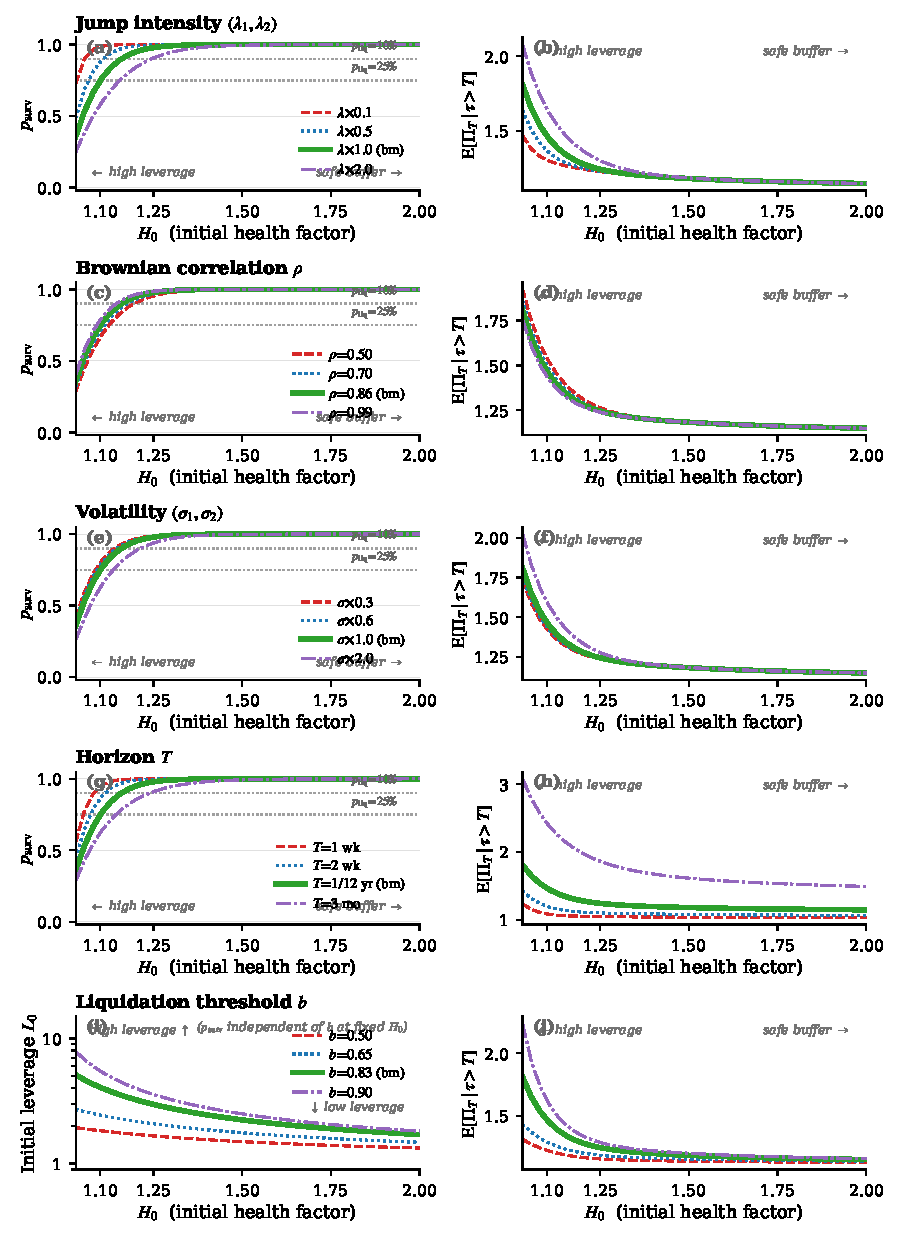
\includegraphics[width=\linewidth,height=0.80\textheight,keepaspectratio]{fig_sensitivity.pdf}
\caption{Left column: survival probability $p_{\mathrm{surv}}$ (rows~a--d) and initial
leverage $L_0$ (row~e, log scale) versus $H_0$. Right column: conditional mean
$\E[\Pi_T\mid\tau>T]$. Each row varies one parameter; all others fixed at
Table~\ref{tab:num-params}. Encoding: colour and line style identify parameter values
(solid/green = benchmark); the heavier line is the baseline.
Laplace--resolvent, $H_0\in[1.031,2.000]$, 40 points per curve.}
\label{fig:sensitivity}
\end{figure}

\clearpage
\subsection{Calibration and sizing uncertainty}\label{sec:calibration-uncertainty}

Pointwise parameter sweeps do not quantify joint sampling variation. We therefore apply a
paired circular moving-block percentile bootstrap to the 540 four-hour return pairs. Each
replicate resamples the same contiguous index blocks for WETH and WBTC, preserving their
contemporaneous pairing and short-range ordering, then repeats ECF calibration, the fixed
AAVE rate adjustment, the fixed terminal-block protocol terms, the fourth-moment admissibility check, and the downstream sizing
rule. The experiment uses 40 replicates, nine-observation blocks (1.5 days), a fixed seed,
and two calibration starts per replicate. All 40 calibrations converged and all 40 sizing
problems were feasible. Two starts make this a tractable uncertainty illustration; the
point calibration itself uses the more extensive 30-start search described in
Appendix~\ref{sec:ecf-init}.

Table~\ref{tab:bootstrap-uncertainty} propagates each recalibration through the rule that
maximizes initial leverage subject to $p_{\mathrm{liq}}\leq0.10$ on the same 200-point
$H_0\in[1.031,2.000]$ grid used below. At the point-selected reference buffer
$H_0=1.163$, survival is $0.905$, while its bootstrap interval is wide. The selected buffer
and leverage also vary materially across recalibrations. By contrast, selected liquidation
probabilities cluster just below 10\% because that is the imposed grid constraint, not
because liquidation risk is precisely estimated.

\begin{table}[ht]
\centering\small
\renewcommand{\arraystretch}{1.2}
\begin{tabular}{lrr}
\toprule
Quantity & Point estimate & 90\% percentile interval \\
\midrule
$p_{\mathrm{surv}}$ at reference $H_0=1.163$ & $0.905$ & $[0.501,\,0.976]$ \\
Selected $H_0$ & $1.163$ & $[1.108,\,1.362]$ \\
Selected initial leverage $L_0$ & $3.496$ & $[2.559,\,3.981]$ \\
Selected $p_{\mathrm{liq}}$ & $0.0954$ & $[0.0927,\,0.0992]$ \\
\bottomrule
\end{tabular}
\caption{Paired circular moving-block bootstrap, conditional on the Kou specification,
penalized ECF criterion, EWM preprocessing, fixed AAVE rates and terminal-block protocol terms, chosen
block length, and discrete sizing grid. These descriptive intervals measure within-model
sampling variability; they are neither model-selection nor out-of-sample forecast
intervals. Script \texttt{jobs/calibration\_uncertainty.py}.}
\label{tab:bootstrap-uncertainty}
\end{table}

\clearpage
